
\setlength{\tabcolsep}{2pt}
\renewcommand{\arraystretch}{0.8}
\begin{figure*}[h!]
	\tiny
	\centering 	\scriptsize
	\begin{tabular}{l|rr|rr|rr|rr||rr|rr|rr|rr||rr|rr|rr|rr}
		& \multicolumn{8}{c}{0.25} & \multicolumn{8}{c}{0.5} & \multicolumn{8}{c}{0.75}\\
		& \multicolumn{2}{c}{C} & \multicolumn{2}{c}{Cnr} & \multicolumn{2}{c}{max} & & & \multicolumn{2}{c}{C} & \multicolumn{2}{c}{Cnr} & \multicolumn{2}{c}{max} & & &  \multicolumn{2}{c}{C} & \multicolumn{2}{c}{Cnr} & \multicolumn{2}{c}{max} & &\\\hline
		& c & t & c & t & c & t & nodes & mugs & c & t & c & t & c & t & nodes & mugs &  c & t & c & t & c & t & nodes & mugs\\\hline
		airport (28) & 0.79 & 0.0017 & 0.79 & 0.0066 & 0.86 & 18.3645 & 7 & 2.05 & 0.54 & 3.5596 & 0.54 & 3.5753 & 0.68 & 3.769 & 5 & 1.47 & 0.29 & 0.0078 & 0.29 & 0.0079 & 0.68 & 0.0035 & 3 & 1\\
		barman (4) & 1 & 0.0047 & 1 & 0.0144 & 1 & 0.0563 & 9 & 3 & 1 & 52.8352 & 1 & 43.8564 & 1 & 8.1814 & 8 & 3 & 0 & - & 0 & - & 1 & - & - & -\\
		blocks (28) & 1 & 0.0001 & 0.93 & 0.0007 & 0.96 & 0.0077 & 393 & 5.69 & 0.96 & 0.0006 & 0.93 & 0.004 & 0.75 & 0.56 & 140 & 6.05 & 0.89 & 0.0077 & 0.86 & 0.0159 & 0.61 & 1.447 & 52 & 6.06\\
		data-network (12) & 0 & - & 0 & - & 1 & - & - & - & 0 & - & 0 & - & 1 & - & - & - & 0 & - & 0 & - & 1 & - & - & -\\
		depot (7) & 1 & 0.0008 & 1 & 0.0043 & 1 & 0.1156 & 38 & 3.71 & 1 & 1.7631 & 1 & 0.7123 & 1 & 10.9838 & 36 & 6.71 & 0.43 & 6.5403 & 0.43 & 1.5582 & 0.57 & 5.8422 & 12 & 2.67\\
		driverlog (13) & 1 & 0.0002 & 1 & 0.0013 & 1 & 0.0432 & 556 & 6.38 & 0.92 & 0.0137 & 0.92 & 0.0374 & 0.77 & 0.3713 & 388 & 13.4 & 0.69 & 3.2144 & 0.69 & 1.9891 & 0.62 & 9.1767 & 191 & 7.88\\
		elevators (40) & 0 & - & 0 & - & 1 & - & - & - & 0 & - & 0 & - & 1 & - & - & - & 0 & - & 0 & - & 0.83 & - & - & -\\
		floortile (13) & 0 & - & 0 & - & 0.46 & - & - & - & 0 & - & 0 & - & 0.15 & - & - & - & 0 & - & 0 & - & 0.15 & - & - & -\\
		freecell (15) & 1 & 0.0003 & 1 & 0.0054 & 1 & 0.15 & 17 & 4 & 0.4 & 0.0085 & 0.47 & 0.0175 & 1 & 0.1357 & 16 & 5.2 & 0 & - & 0 & - & 0.93 & - & - & -\\
		ged (15) & 0 & - & 0 & - & 0.67 & - & - & - & 0 & - & 0 & - & 0.67 & - & - & - & 0 & - & 0 & - & 0.67 & - & - & -\\
		grid (2) & 1 & 0.0002 & 1 & 0.0034 & 1 & 0.0138 & 6 & 1.5 & 1 & 0.0122 & 1 & 0.0177 & 1 & 1.2066 & 6 & 1.5 & 0.5 & 0.0018 & 1 & 0.004 & 1 & 0.02 & 3 & 1\\
		gripper (7) & 0.71 & 0.0079 & 0.71 & 0.0069 & 0.71 & 0.0172 & 1087 & 77.4 & 0.57 & 1.0907 & 0.57 & 0.1444 & 0.57 & 0.0733 & 286 & 87 & 0.43 & 1.4578 & 0.43 & 0.8578 & 0.71 & 0.0336 & 43 & 12.67\\
		hiking (9) & 1 & 0.0019 & 1 & 0.0029 & 1 & 0.1407 & 4 & 1.44 & 0.67 & 0.4672 & 0.67 & 0.3678 & 1 & 3.9923 & 4 & 1.67 & 0.22 & 2.5099 & 0.22 & 1.1453 & 1 & 0.9072 & 4 & 1\\
		logistics (26) & 1 & 0.0007 & 1 & 0.0036 & 0.85 & 4.5539 & 110 & 4.05 & 0.77 & 0.1136 & 0.85 & 0.0671 & 0.58 & 5.1033 & 48 & 4.53 & 0.54 & 0.3488 & 0.58 & 0.1775 & 0.46 & 0.2939 & 22 & 2.17\\
		miconic (141) & 0.47 & 0.0016 & 0.46 & 0.0044 & 0.4 & 0.0477 & 438 & 27.89 & 0.29 & 0.3027 & 0.35 & 0.0338 & 0.32 & 0.1269 & 66 & 17.78 & 0.25 & 0.9975 & 0.28 & 0.1975 & 0.32 & 0.091 & 20 & 5.54\\
		mprime (22) & 1 & 0.0002 & 1 & 0.0036 & 1 & 0.0115 & 4 & 1.32 & 1 & 0.0011 & 1 & 0.0044 & 1 & 0.3336 & 4 & 1.23 & 1 & 0.0167 & 1 & 0.026 & 1 & 16.9777 & 4 & 1.18\\
		mystery (17) & 1 & 0.0003 & 1 & 0.0052 & 1 & 0.0199 & 4 & 1.41 & 1 & 0.0018 & 1 & 0.0062 & 1 & 1.6016 & 4 & 1.35 & 0.82 & 0.0049 & 0.82 & 0.0134 & 0.88 & 1.513 & 4 & 1.15\\
		nomystery (14) & 0.71 & 0.0003 & 0.71 & 3 & 1 & 0.0321 & 76 & 5.4 & 0 & - & 0.07 & - & 0.71 & - & - & - & 0 & - & 0 & - & 0.57 & - & - & -\\
		openstacks (47) & 0.15 & 0.0016 & 0.15 & 24 & 0.51 & 0.1372 & 316 & 6.43 & 0.11 & 0.0177 & 0.11 & 0.0372 & 0.47 & 0.0163 & 33 & 4.2 & 0.11 & - & 0 & - & 0.43 & - & - & -\\
		org-syn (7) & 1 & 0.0002 & 0.86 & 0.0179 & 0.86 & 0.0486 & 40 & 3.17 & 1 & 0.0011 & 0.86 & 0.0198 & 0.86 & 0.0504 & 40 & 3.17 & 1 & 0.0013 & 0.86 & 0.0208 & 0.86 & 0.054 & 40 & 3.17\\
		org-syn-s (10) & 0.8 & 0.0007 & 0.6 & 0.0152 & 0.6 & 5.9967 & 64 & 3.17 & 0.5 & 0.0004 & 0.5 & 0.0062 & 0.6 & 0.0374 & 70 & 3 & 0.2 & 0.0003 & 0.2 & 0.0072 & 0.6 & 0.0293 & 129 & 6\\
		parcprinter (24) & 0 & - & 0 & - & 0.42 & - & - & - & 0 & - & 0 & - & 0.42 & - & - & - & 0 & - & 0 & - & 0.42 & - & - & -\\
		parking (5) & 1 & - & 0 & - & 0 & - & - & - & 0.2 & - & 0 & - & 0 & - & - & - & 0 & - & 0 & - & 0 & - & - & -\\
		pathways-noneg (5) & 1 & 0.0002 & 1 & 0.0009 & 1 & 1.5975 & 20 & 3.2 & 0.4 & 0.0002 & 0.4 & 0.0002 & 0.8 & 0.0043 & 4 & 1.5 & 0.2 & 0.0001 & 0.2 & 0.0002 & 0.8 & 0.0022 & 3 & 1\\
		pegsol (2) & 0 & - & 0 & - & 0 & - &  &  & 0 & - & 0 & - & 0 & - & - & - & 0 & - & 0 & - & 0 & - & - & -\\
		pipesworld-nt (17) & 1 & 0.0006 & 1 & 4 & 1 & 0.0336 & 40 & 3.35 & 0.94 & 0.5306 & 0.94 & 0.3581 & 0.94 & 1.7601 & 26 & 5 & 0.82 & 10.0899 & 0.82 & 13.0619 & 0.94 & 41.5442 & 18 & 4.14\\
		pipesworld-t (12) & 0.92 & 0.0003 & 0.92 & 4 & 1 & 0.0809 & 34 & 3.45 & 0.92 & 0.2643 & 0.92 & 0.2918 & 0.92 & 11.8348 & 31 & 5 & 0.75 & 0.4525 & 0.75 & 0.6277 & 0.75 & 18.627 & 15 & 3.13\\
		psr-small (49) & 1 & 0.0002 & 0.98 & 0.0007 & 0.98 & 0.0006 & 615 & 3.44 & 1 & 0.0009 & 0.98 & 0.0035 & 0.98 & 0.004 & 475 & 2.52 & 0.96 & 0.0055 & 0.92 & 0.0135 & 0.96 & 0.0637 & 83 & 1.78\\
		rovers (8) & 1 & 0.0097 & 1 & 0.0031 & 1 & 0.0873 & 163 & 18 & 0.88 & 0.6903 & 0.88 & 0.0918 & 0.88 & 1.8094 & 34 & 11.43 & 0.5 & 0.0016 & 0.88 & 0.0018 & 0.75 & 0.0024 & 6 & 1.5\\
		satellite (7) & 1 & 0.0002 & 1 & 0.0027 & 1 & 0.3211 & 176 & 5.57 & 0.86 & 0.0417 & 1 & 0.0461 & 0.86 & 1.2065 & 114 & 18.67 & 0.71 & 0.2023 & 0.86 & 0.1006 & 0.57 & 0.1612 & 51 & 13.25\\
		scanalyzer (23) & 0.57 & 0.0001 & 0.39 & 0.0012 & 0.39 & 0.0103 & 2359 & 12.67 & 0.39 & 0.0476 & 0.39 & 0.0198 & 0.39 & 0.1573 & 1939 & 45.78 & 0.22 & 0.131 & 0.22 & 0.0369 & 0.39 & 0.1435 & 550 & 30.8\\
		snake (7) & 0.57 & 0.0008 & 0.14 & 0.0151 & 0.14 & 0.1996 & 245 & 4 & 0 & - & 0 & - & 0.14 & - & - & - & 0 & - & 0 & - & 0.14 & - & - & -\\
		sokoban (50) & 0 & - & 0 & - & 0.98 & - & - & - & 0 & - & 0 & - & 0.94 & - & - & - & 0 & - & 0 & - & 0.84 & - & - & -\\
		storage (15) & 1 & 0.0003 & 1 & 1 & 1 & 0.0025 & 13 & 3.6 & 1 & 0.2554 & 1 & 0.0665 & 1 & 0.1762 & 11 & 3.73 & 0.93 & 9.902 & 0.93 & 3.744 & 1 & 0.9675 & 7 & 1.93\\
		termes (6) & 1 & 0.0008 & 0.33 & 0.0469 & 1 & 36 & 2881 & 2.5 & 0.17 & - & 0 & - & 0.17 & - & - & - & 0 & - & 0 &  & 0 & - & - & -\\
		tetris (6) & 0.83 & 0.0003 & 0.33 & 0.0088 & 0.33 & 0.0147 & 257 & 6.5 & 0.5 & 0.0133 & 0.33 & 0.0297 & 0.33 & 0.0307 & 205 & 10 & 0.33 & 0.8305 & 0.33 & 0.5429 & 0.5 & 0.1313 & 106 & 5.5\\
		tidybot (23) & 1 & 0.0032 & 1 & 0.0536 & 1 & 1.4659 & 16 & 2.57 & 0.7 & 3.9946 & 0.7 & 3.3744 & 1 & 34.3564 & 16 & 3 & 0.43 & 7.1982 & 0.3 & 10.1166 & 0.3 & 14.7701 & 15 & 3.5\\
		tpp (7) & 1 & 0.0002 & 1 & 1 & 1 & 24 & 37 & 3.86 & 1 & 0.0328 & 1 & 0.0201 & 0.86 & 0.2812 & 21 & 6.17 & 0.71 & 0.0469 & 0.86 & 0.0242 & 0.86 & 0.014 & 9 & 2.8\\
		transport (23) & 1 & 0.0004 & 1 & 0.0015 & 1 & 0.0154 & 17 & 3.04 & 1 & 0.0649 & 1 & 0.1057 & 1 & 1.0104 & 16 & 3.17 & 0.96 & 6.7547 & 0.96 & 4.1551 & 1 & 14.8687 & 12 & 2.05\\
		trucks (10) & 0.2 & 0.0001 & 0.2 & 0.0003 & 1 & 0.0012 & 13 & 3.5 & 0 & - & 0 & - & 0.6 & - & - & - & 0 & - & 0 & - & 0.6 & - & - & -\\
		visitall (14) & 0.71 & 0.0001 & 0.57 & 0.0002 & 0.64 & 0.0004 & 10292 & 19.88 & 0.71 & 0.0002 & 0.5 & 0.0013 & 0.57 & 0.0046 & 6930 & 38 & 0.57 & 0.0034 & 0.5 & 0.0087 & 0.5 & 0.0338 & 4533 & 38.29\\
		woodworking (29) & 0.45 & 0.0001 & 0.17 & 0.0006 & 0.24 & 0.0016 & 2148 & 17.8 & 0.1 & 0.0012 & 0.1 & 0.0058 & 0.17 & 0.0134 & 1426 & 29 & 0.07 & 0.0097 & 0.1 & 0.0802 & 0.17 & 0.1136 & 1093 & 17\\
		zenotravel (13) & 1 & 0.0008 & 1 & 0.0073 & 0.92 & 0.2413 & 122 & 8 & 0.69 & 0.0011 & 0.77 & 0.0045 & 0.62 & 0.0424 & 38 & 3.75 & 0.69 & 0.4634 & 0.69 & 0.3243 & 0.62 & 1.6294 & 26 & 2.38\\\hline
		(862) & 0.62 & 0.0012 & 0.58 & 0.0077 & 0.76 & 0.9414 & 632 & 8.05 & 0.48 & 2.0666 & 0.49 & 1.6665 & 0.68 & 2.7886 & 392 & 11.97 & 0.39 & 1.7662 & 0.39 & 1.3409 & 0.62 & 4.4643 & 245 & 6.95\\
	\end{tabular}

 
        \vspace{-0.2cm}
	\caption{Empirical results on IPC benchmarks modified for oversubscription planning. Reference Points: comparison performance for classical planning problems (see discussion in text). Coverage: coverage of our MUGS algorithms SysS and SysW, with vs.\ without conjunction learning \hc. \# MUGS: Average number of MUGS per domain, indicating explanation size (see text). Search Tree Fraction: fraction of worst-case search tree explored by SysS and SysW. Best performance in each part shown in \textbf{boldface}. Cost bounds set to $x$ times optimal cost.}
	\label{table:coverage_ipc}
        \vspace{-0.4cm}
\end{figure*}

\section{An Illustrative Example}
\label{illustrative-example}


%% Loading and unloading costs no fuel, while driving costs between 1 and
%% 5 fuels units (as indicated by edge labels).\\ The amount of fuel
%% available is 1.5 times higher than needed to deliver all packages;
%% concretely, the initial fuel in trucks is $fuel(T_0) = 16$, $fuel(T_1)
%% = 7$.

To illustrate our approach and the kind of answers it provides to user
questions, let us briefly consider the IPC NoMystery domain, a
classical transportation domain with fuel
consumption. Figure~\ref{fig:nomystery-example} illustrates an example
instance with two trucks and three packages. Fuel costs are indicated
at road segments (initial fuel is $16$ for $T_0$ and $7$ for
$T_1$). All packages are initially at $L_0$ (shown in blue); they need
to be delivered to individual goal locations (shown in red).

\begin{wrapfigure}{r}{0.5\columnwidth}
\vspace{-0.4cm} \hspace{-0.4cm} 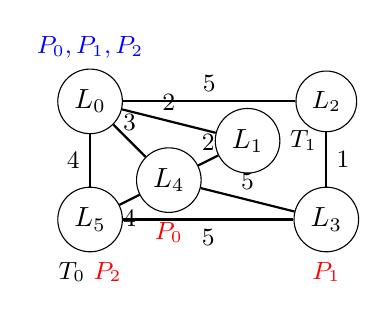
\begin{tikzpicture}[scale=0.5]
  \node[draw, circle, label=above:{\small \textcolor{blue}{$P_0, P_1,P_2$}}] (l0) at (0,0) {$L_0$};
  \node[draw, circle, label=right:{\small $T_1$}] (l1) at (4,-1) {$L_1$};
  \node[draw, circle] (l2) at (6,0) {\small $L_2$};
  \node[draw, circle, label=below:{\small \textcolor{red}{$P_1$}}] (l3) at (6,-3) {$L_3$};
  \node[draw, circle, label=below:{\small \textcolor{red}{$P_0$}}] (l4) at (2,-2) {$L_4$};
  \node[draw, circle, label=below:{\small $T_0$ \textcolor{red}{$P_2$}}] (l5) at (0,-3) {$L_5$};

  \draw[thick] (l0) to node[above] {\small 5} (l2);
  \draw[thick] (l0) to node[above] {\small 2} (l1);
  \draw[thick] (l0) to node[above] {\small 3} (l4);
  \draw[thick] (l0) to node[left] {\small 4} (l5);
  \draw[thick] (l2) to node[right] {\small 1} (l3);
  \draw[thick] (l4) to node[above] {\small 2} (l1);
  \draw[thick] (l4) to node[above] {\small 5} (l3);
  \draw[thick] (l5) to node[below] {\small 5} (l3);
  \draw[thick] (l4) to node[below] {\small 4} (l5);
\end{tikzpicture}
\vspace{-0.2cm}
\hspace{-0.6cm} \caption{Illustrative IPC NoMystery example.}
\label{fig:nomystery-example}
\vspace{-0.2cm}
\end{wrapfigure}

We define three kinds of action-set properties for this domain:
\emph{uses $T_i$ $(L_x,L_y)$} (truck $T_i$ drives at least once from
$L_x$ to $L_y$ or vice versa); \emph{doesn't use $T_i$ $(L_x,L_y)$}
(truck $T_i$ does not drive from $L_x$ to $L_y$ or vice versa);
\emph{same truck $P_x$ $P_y$} (both packages are delivered by the same
truck). We consider six instances of these properties: 1.\ uses $T_0$
$(L_2,L_3)$; 2.\ same truck $P_1$ $P_2$; 3.\ uses $T_0$ $(L_4,L_3)$;
4.\ same truck $P_2$ $P_0$; 5.\ doesn't use $T_0$ $(L_0,L_5)$;
6.\ uses $T_1$ $(L_5,L_4)$.

Fixing the package destinations as hard goals (defining the set of
plans \plans\ considered), and computing the MUGS over these six
action-set properties using the algorithms previously described, it
turns out there are 7 minimal unsolvable subsets of these properties,
each of size 3.

Say now that the current plan uses $T_0$ only, and includes the action
(drive T0 L5 L0). The user might ask \emph{''Why don't you avoid the
  road $L_0-L_5$, which has a lot of traffic at the
  moment?''}. Answering this question in terms of contrastive
explanation, as previously discussed, corresponds to forcing property
5 to be satisfied. At the same time, the plan already satisfies
properties 2 and 4. However, one of the MUGS is $\{2,4,5\}$, and hence
the answer to the user question would be: \textit{Because if you don't
  use that road, then you would not be able to deliver all packages
  using a single truck}.
